\documentclass{standalone}
\usepackage{tikz}
\usetikzlibrary{patterns, positioning}
\usetikzlibrary{shapes.misc}
\usepackage[outline]{contour}
\contourlength{1.5pt} 
\usepackage[sfdefault]{ClearSans} %% option 'sfdefault' activates Clear Sans as the default text font
\usepackage[T1]{fontenc}

\begin{document}
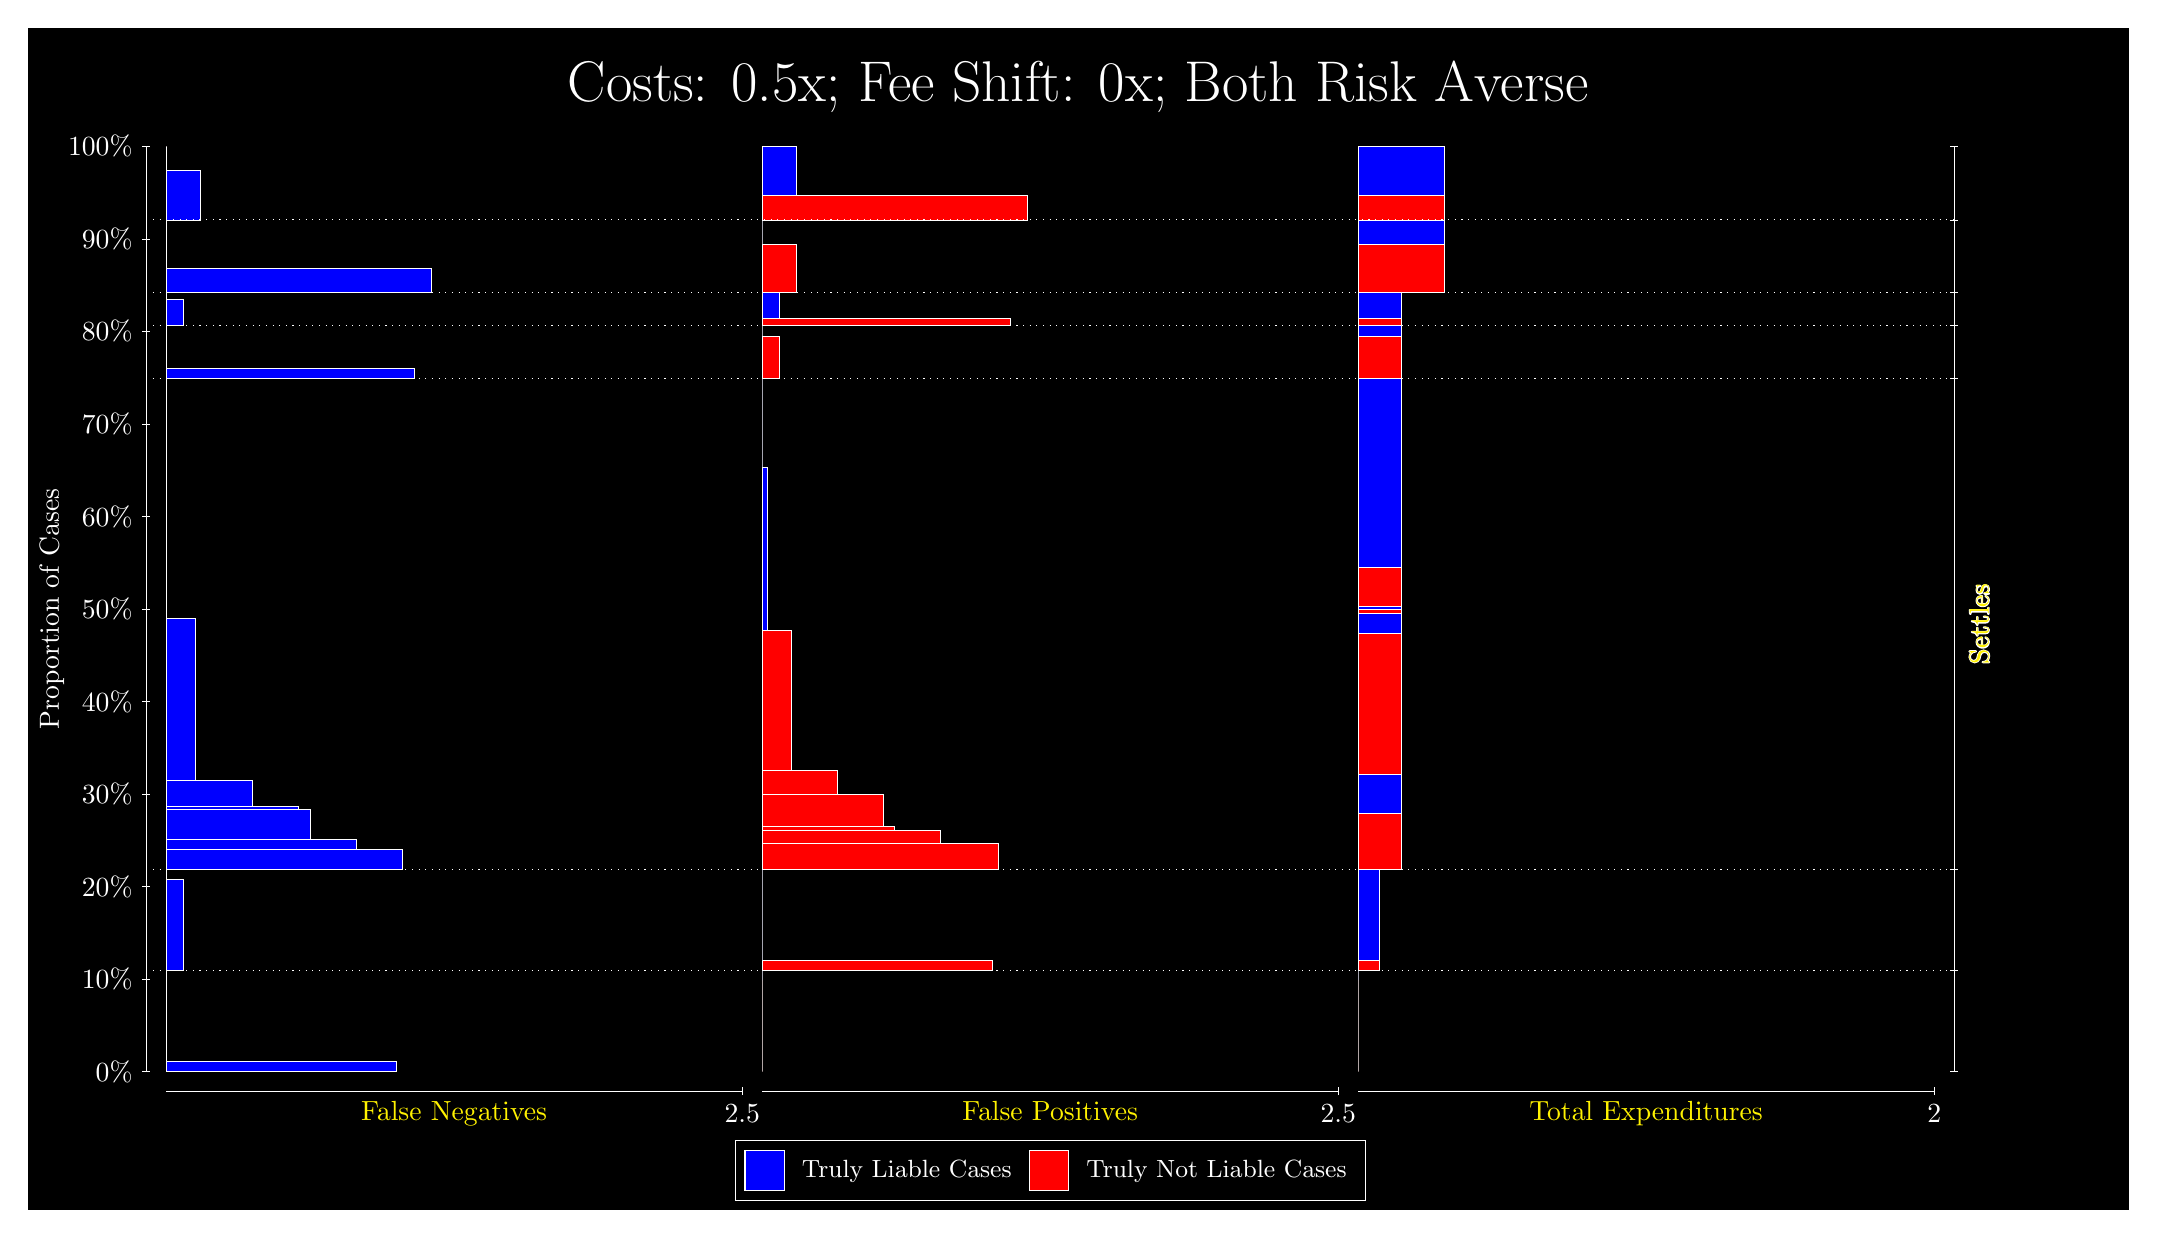
\begin{tikzpicture}
\draw[fill=black] (0,0) rectangle (26.667,15);
\draw[text=white] (0,13.5) rectangle (26.667,15) node[midway] {\huge Costs: 0.5x; Fee Shift: 0x; Both Risk Averse};
\draw[white, very thin] (1.5,1.75) -- (1.5,13.5);
\node[rotate=90, text=white, anchor=center] at (0.3, 7.625) {Proportion of Cases};
\draw[white, very thin] (1.45,1.75) -- (1.55,1.75);
\node[text=white, anchor=east] at (1.45, 1.75) {0\%};
\draw[white, very thin] (1.45,2.925) -- (1.55,2.925);
\node[text=white, anchor=east] at (1.45, 2.925) {10\%};
\draw[white, very thin] (1.45,4.1) -- (1.55,4.1);
\node[text=white, anchor=east] at (1.45, 4.1) {20\%};
\draw[white, very thin] (1.45,5.275) -- (1.55,5.275);
\node[text=white, anchor=east] at (1.45, 5.275) {30\%};
\draw[white, very thin] (1.45,6.45) -- (1.55,6.45);
\node[text=white, anchor=east] at (1.45, 6.45) {40\%};
\draw[white, very thin] (1.45,7.625) -- (1.55,7.625);
\node[text=white, anchor=east] at (1.45, 7.625) {50\%};
\draw[white, very thin] (1.45,8.8) -- (1.55,8.8);
\node[text=white, anchor=east] at (1.45, 8.8) {60\%};
\draw[white, very thin] (1.45,9.975) -- (1.55,9.975);
\node[text=white, anchor=east] at (1.45, 9.975) {70\%};
\draw[white, very thin] (1.45,11.15) -- (1.55,11.15);
\node[text=white, anchor=east] at (1.45, 11.15) {80\%};
\draw[white, very thin] (1.45,12.325) -- (1.55,12.325);
\node[text=white, anchor=east] at (1.45, 12.325) {90\%};
\draw[white, very thin] (1.45,13.5) -- (1.55,13.5);
\node[text=white, anchor=east] at (1.45, 13.5) {100\%};

\draw[white, very thin] (24.457,1.75) -- (24.457,13.5);
\draw[white, very thin] (24.407,1.75) -- (24.507,1.75);
\node[anchor=west] at (24.407, 1.75) {};
\draw[white, very thin] (24.407,3.034) -- (24.507,3.034);
\node[anchor=west] at (24.407, 3.034) {};
\draw[white, very thin] (24.407,4.3173) -- (24.507,4.3173);
\node[anchor=west] at (24.407, 4.3173) {};
\draw[white, very thin] (24.407,10.549) -- (24.507,10.549);
\node[anchor=west] at (24.407, 10.549) {};
\draw[white, very thin] (24.407,11.224) -- (24.507,11.224);
\node[anchor=west] at (24.407, 11.224) {};
\draw[white, very thin] (24.407,11.642) -- (24.507,11.642);
\node[anchor=west] at (24.407, 11.642) {};
\draw[white, very thin] (24.407,12.567) -- (24.507,12.567);
\node[anchor=west] at (24.407, 12.567) {};
\draw[white, very thin] (24.407,13.5) -- (24.507,13.5);
\node[anchor=west] at (24.407, 13.5) {};

\draw[white, very thin, fill=blue] (1.75,1.75) rectangle (4.6775,1.8744);
\draw[white, very thin, fill=red] (1.75,1.8744) rectangle (1.75,3.034);
\draw[white, very thin, fill=blue] (1.75,3.034) rectangle (1.9696,4.1933);
\draw[white, very thin, fill=red] (1.75,4.1933) rectangle (1.75,4.3173);
\draw[white, very thin, fill=blue] (1.75,4.3173) rectangle (4.7507,4.5718);
\draw[white, very thin, fill=blue] (1.75,4.5718) rectangle (4.1652,4.6937);
\draw[white, very thin, fill=blue] (1.75,4.6937) rectangle (3.5797,5.0756);
\draw[white, very thin, fill=blue] (1.75,5.0756) rectangle (3.4333,5.1188);
\draw[white, very thin, fill=blue] (1.75,5.1188) rectangle (2.8478,5.4438);
\draw[white, very thin, fill=blue] (1.75,5.4438) rectangle (2.1159,7.5119);
\draw[white, very thin, fill=red] (1.75,7.5119) rectangle (1.75,10.549);
\draw[white, very thin, fill=blue] (1.75,10.549) rectangle (4.8971,10.683);
\draw[white, very thin, fill=red] (1.75,10.683) rectangle (1.75,11.224);
\draw[white, very thin, fill=blue] (1.75,11.224) rectangle (1.9696,11.555);
\draw[white, very thin, fill=red] (1.75,11.555) rectangle (1.75,11.642);
\draw[white, very thin, fill=blue] (1.75,11.642) rectangle (5.1167,11.95);
\draw[white, very thin, fill=red] (1.75,11.95) rectangle (1.75,12.567);
\draw[white, very thin, fill=blue] (1.75,12.567) rectangle (2.1891,13.19);
\draw[white, very thin, fill=red] (1.75,13.19) rectangle (1.75,13.5);
\draw[white, very thin, fill=red] (9.3189,1.75) rectangle (9.3189,2.9097);
\draw[white, very thin, fill=blue] (9.3189,2.9097) rectangle (9.3189,3.034);
\draw[white, very thin, fill=red] (9.3189,3.034) rectangle (12.246,3.158);
\draw[white, very thin, fill=blue] (9.3189,3.158) rectangle (9.3189,4.3173);
\draw[white, very thin, fill=red] (9.3189,4.3173) rectangle (12.32,4.6496);
\draw[white, very thin, fill=red] (9.3189,4.6496) rectangle (11.588,4.8131);
\draw[white, very thin, fill=red] (9.3189,4.8131) rectangle (11.002,4.8626);
\draw[white, very thin, fill=red] (9.3189,4.8626) rectangle (10.856,5.2774);
\draw[white, very thin, fill=red] (9.3189,5.2774) rectangle (10.27,5.57);
\draw[white, very thin, fill=red] (9.3189,5.57) rectangle (9.6848,7.3547);
\draw[white, very thin, fill=blue] (9.3189,7.3547) rectangle (9.3921,9.4228);
\draw[white, very thin, fill=blue] (9.3189,9.4228) rectangle (9.3189,10.549);
\draw[white, very thin, fill=red] (9.3189,10.549) rectangle (9.5384,11.091);
\draw[white, very thin, fill=blue] (9.3189,11.091) rectangle (9.3189,11.224);
\draw[white, very thin, fill=red] (9.3189,11.224) rectangle (12.466,11.311);
\draw[white, very thin, fill=blue] (9.3189,11.311) rectangle (9.5384,11.642);
\draw[white, very thin, fill=red] (9.3189,11.642) rectangle (9.758,12.259);
\draw[white, very thin, fill=blue] (9.3189,12.259) rectangle (9.3189,12.567);
\draw[white, very thin, fill=red] (9.3189,12.567) rectangle (12.686,12.877);
\draw[white, very thin, fill=blue] (9.3189,12.877) rectangle (9.758,13.5);
\draw[white, very thin, fill=red] (16.888,1.75) rectangle (16.888,2.9097);
\draw[white, very thin, fill=blue] (16.888,2.9097) rectangle (16.888,3.034);
\draw[white, very thin, fill=red] (16.888,3.034) rectangle (17.162,3.158);
\draw[white, very thin, fill=blue] (16.888,3.158) rectangle (17.162,4.3173);
\draw[white, very thin, fill=red] (16.888,4.3173) rectangle (17.437,5.0246);
\draw[white, very thin, fill=blue] (16.888,5.0246) rectangle (17.437,5.5285);
\draw[white, very thin, fill=red] (16.888,5.5285) rectangle (17.437,7.3132);
\draw[white, very thin, fill=blue] (16.888,7.3132) rectangle (17.437,7.5678);
\draw[white, very thin, fill=red] (16.888,7.5678) rectangle (17.437,7.6173);
\draw[white, very thin, fill=blue] (16.888,7.6173) rectangle (17.437,7.6604);
\draw[white, very thin, fill=red] (16.888,7.6604) rectangle (17.437,8.1563);
\draw[white, very thin, fill=blue] (16.888,8.1563) rectangle (17.437,10.549);
\draw[white, very thin, fill=red] (16.888,10.549) rectangle (17.437,11.091);
\draw[white, very thin, fill=blue] (16.888,11.091) rectangle (17.437,11.224);
\draw[white, very thin, fill=red] (16.888,11.224) rectangle (17.437,11.311);
\draw[white, very thin, fill=blue] (16.888,11.311) rectangle (17.437,11.642);
\draw[white, very thin, fill=red] (16.888,11.642) rectangle (17.986,12.259);
\draw[white, very thin, fill=blue] (16.888,12.259) rectangle (17.986,12.567);
\draw[white, very thin, fill=red] (16.888,12.567) rectangle (17.986,12.877);
\draw[white, very thin, fill=blue] (16.888,12.877) rectangle (17.986,13.5);
\draw[white, dotted] (1.5,3.034) -- (24.457,3.034);
\draw[white, dotted] (1.5,4.3173) -- (24.457,4.3173);
\draw[white, dotted] (1.5,10.549) -- (24.457,10.549);
\draw[white, dotted] (1.5,11.224) -- (24.457,11.224);
\draw[white, dotted] (1.5,11.642) -- (24.457,11.642);
\draw[white, dotted] (1.5,12.567) -- (24.457,12.567);
\draw[white, very thin] (1.75,1.5) -- (9.0689,1.5);
\node[text=yellow, anchor=north] at (5.4094, 1.5) {False Negatives};
\draw[white, very thin] (9.0689,1.45) -- (9.0689,1.55);
\node[text=white, anchor=north] at (9.0689, 1.45) {2.5};

\draw[white, very thin] (9.3189,1.5) -- (16.638,1.5);
\node[text=yellow, anchor=north] at (12.978, 1.5) {False Positives};
\draw[white, very thin] (16.638,1.45) -- (16.638,1.55);
\node[text=white, anchor=north] at (16.638, 1.45) {2.5};

\draw[white, very thin] (16.888,1.5) -- (24.207,1.5);
\node[text=yellow, anchor=north] at (20.547, 1.5) {Total Expenditures};
\draw[white, very thin] (24.207,1.45) -- (24.207,1.55);
\node[text=white, anchor=north] at (24.207, 1.45) {2};



\node[text=yellow, centered, rotate=90] at (24.777, 7.4333) {\contour{white}{Settles}};





\draw (12.978300999999998,1.5) node[draw=none] (baseCoordinate) {};
\begin{scope}[align=center]
        \matrix[scale=0.5, draw=white, below=0.5cm of baseCoordinate, nodes={draw}, column sep=0.1cm]{
            \node[rectangle, draw, minimum width=0.5cm, minimum height=0.5cm, fill=blue] {}; &
            \node[draw=none, font=\small, text=white] (B) {Truly Liable Cases}; &
            \node[rectangle, draw, minimum width=0.5cm, minimum height=0.5cm, fill=red] {}; &
            \node[draw=none, font=\small, text=white] (B) {Truly Not Liable Cases}; \\
            };
\end{scope}

\end{tikzpicture}
\end{document}